\chapter{Tutorial programs}

This release of SISL is bundled with a number of sample programs which are intended
to make the user more familiar with the use of the API, as well as demonstrating 
some of its capabilities.  

\section{Compiling the programs}
Makefiles are provided to compile all provided source code, included the sample programs.
Refer to (\ref{compile}) for details on using the provided makefiles.  Please note 
that since these executables link both with SISL 4.4 and the `streaming' library, these 
must be compiled first.\\

The compilation of the example code has been verified for the GCC 3.3.3 compiler 
and the Microsoft Visual C++ .NET 2002 compiler, but it should be general enough to 
compile relatively troublefree on most platforms.

\section{Description and commentaries on the sample programs}

The example programs are named \verb/example01/ through \verb/example15/.  Each of the
program demonstrates the use of a single or a couple of SISL functions.  The programs
produces output files that contain geometric objects in the \verb/Go/-format, which 
can then be visualised by the provided KRULL-viewer.  

To keep things as simple as possible, the example programs (with the exception of
\verb/example15/) take no command line arguments.  Instead, upon execution they inform
the user about what they are about to do, and which files will be read from and written
to.  The names of the input and output files are hard-coded in each example, but the
user can experiment by changing the name of these files if she wants to.  Several of
the sample programs rely upon files generated by earlier examples, so the user should 
make sure she runs through them in chronological order.

\subsection{example01.C}

\subsubsection{What it does}
This program demonstrates how to directly specify a spline curve by providing the 
position of control points and a knotvector (parametrization).  It generates such
a curve by using hard-coded values as input to the SISL  \verb/newCurve/ routine.
\subsubsection{What it demonstrates}
\begin{enumerate}
\item How control points and knotvectors are specified in memory
\item How to use the \verb/newCurve/ routine
\item How to clean up memory using \verb/freeCurve/
\end{enumerate}

\subsubsection{Input/output}
The program takes no input files.\\
The program generates the files \verb/example1_curve.g2/ and \verb/example1_points.g2/.
The former contains the curve object and the latter contains the control points, expressed
in the \verb/Go/-format.

\subsection{example02.C}

\subsubsection{What it does}
This program demonstrates one of the simplest \emph{interpolation} cases for spline 
curves in SISL.  A sequence of 6 3D-points are provided (hardcoded), and the routine
generates a spline curve that fits exactly through these points.  Note that this is a
simple example of a more general routine, which can also take into consideration
tangents, end point conditions, etc.

\subsubsection{What it demonstrates}
\begin{enumerate}
\item The use of the SISL routine \verb/s1356/ for interpolating points with a curve
\end{enumerate}
\subsubsection{Input/output}
The program takes no input files.\\
The program generates the file \verb/example2_points.g2/ and \verb/example2_curve.g2/.
The first file contains the points to be interpolated, and the second file contains the
generated curve.

\subsection{example03.C}

\subsubsection{What it does}
This program creates a so-called \emph{blend-curve} between two other curves, creating a
smooth connection between these.  In this program, the blend curve connects the \emph{end 
points} of the two other curves, but in its generality, the routine can be used to create 
blend curves connecting to any point on the other curves.

\subsubsection{What it demonstrates}
\begin{enumerate}
\item What a blend curve is and how it can be specified
\item The use of the SISL routine \verb/s1606/ which computes the blend curve
\item The use of the SISL routine \verb/s1227/ which evaluates points (and derivatives)
on a spline curve
\item How to directly access data members of the \verb/SISLCurve/ struct.
\end{enumerate}
\subsubsection{Input/output}
The program takes as input the files \verb/example1_curve.g2/ and \verb/example2_points.g2/,
which are respectively generated by the programs \verb/example01/ and \verb/example02/.
The generated blend curve will be saved to the file \verb/example3_curve.g2/.

\subsection{example04.C}

\subsubsection{What it does}
This program generates an \emph{offset curve} from another curve.  An offset curve is
specified as having a fixed distance in a specified direction from the original curve.
The generated offset curve will not be exact, as this would in general be impossible using
spline-function.  We can however obtain an approximation within a user-specified tolerance.

\subsubsection{What it demonstrates}
\begin{enumerate}
\item What an offset curve is and how it can be specified
\item The way in which many SISL routines deal with geometric tolerances
\item The use of the SISL routine \verb/s1360/ which computes the offset curve within a 
specified, geometric tolerance
\end{enumerate}
\subsubsection{Input/output}
The original curve is read from the file \verb/example1_curve.g2/, which is generated by
the program \verb/example01/.  The resulting approximation of the offset curve will be 
written to the file \verb/example4_curve.g2/.

\subsection{example05.C}

\subsubsection{What it does}
This program generates a family of conic section curves, which are represented as rational
splines.  Conic sections can be \emph{exactly} represented with such splines, so no geometric 
tolerance specification is needed.  The program will generate three ellipse segments, one
parabola segment and three hyperbola segments, based on internal, hard-coded data.

\subsubsection{What it demonstrates}
\begin{enumerate}
\item The use of the SISL routine \verb/s1011/ to generate all kinds of conic sections
\item The important fact that conic sections can be exactly represented by rational splines
\item How a single \emph{shape} parameter can specify whether the generated curve will be an
ellipse, a parabola or a hyperbola
\end{enumerate}
\subsubsection{Input/output}
The program takes no input files.\\
The program generates the file \verb/example5_curve.g2/ which contains all the generated curves.

\subsection{example06.C}

\subsubsection{What it does}
This program generates two curves (from internal, hardcoded data), and computes their 
intersections.  Computation of intersections is an extremely important part of SISL, although 
the intersection of two curves is a minor problem in this respect.
\subsubsection{What it demonstrates}
\begin{enumerate}
\item The use of the SISL routine \verb/s1857/ for computing the intersection points between
two given spline curves
\item Underlines the fact that the detected intersection points are returned as parameter values,
and have to be evaluated in order to find their 3D positions
\item How to clean up an array of intersection curves (SISLIntcurve), although, in 
this example, this array will already be empty
\end{enumerate}
\subsubsection{Input/output}
The program takes no input files (the data for the curves is hard-coded).  \\
The generated curves will be written to the files \verb/example6_curve_1.g2/ and \\
\verb/example6_curve_2.g2/.  The intersection point positions will be written to the file
\verb/example6_isectpoints.g2/.

\subsection{example07.C}

\subsubsection{What it does}
This is a very short and simple program that calculates the arc length of a curve.
\subsubsection{What it demonstrates}
\begin{enumerate}
\item The use of the SISL routine \verb/s1240/ for computing the length of a spline curve
\end{enumerate}
\subsubsection{Input/output}
The curve whose length is calculated is read from the file \verb/example6_curve_1/, which
has been generated by the sample program \verb/example06/.  The calculated length will be
written to standard output.

\subsection{example08.C}

\subsubsection{What it does}
This program generates two non-intersecting spline curves (from internal, hard-coded cata), and
computes their mutual closest point.  The call is very similar to the one in \verb/example06/, 
where we wanted to compute curve intersections.
\subsubsection{What it demonstrates}
\begin{enumerate}
\item The use of the SISL routine \verb/s1955/ for locating the closest points of two curves.
\end{enumerate}
\subsubsection{Input/output}
As the curves are specified directly by internal data, no input files are needed.\\
The two generated curves will be saved to the two files \verb/example8_curve_1.g2/ and 
\verb/example8_curve_2.g2/.  The closest points will be written to the file \\
\verb/example8_closestpoints.g2/.

\subsection{example09.C}

\subsubsection{What it does}
This program generates four different surfaces interpolating an array of spatial points.  
The surfaces have different spline order, so that even though they interpolate the same 
points, they have different shapes.
\subsubsection{What it demonstrates}
\begin{enumerate}
\item The use of the SISL routine \verb/s1537/ for generating an interpolating surface to a grid
of points
\item The effect of the spline order on the interpolating surface
\end{enumerate}
\subsubsection{Input/output}
The program takes no input files (the points to be interpolated are hard-coded). \\
The program creates two data files: \verb/example9_points.g2/, which contains all the 
interpolated points, and \verb/example9_surf.g2/, which contains the four generated
surfaces.

\subsection{example10.C}

\subsubsection{What it does}
This program generates a sequence of spline curves.  Moreover, it generates a \emph{lofted
surface} interpolating these curves.  The lofted surface has the original sequence of curves
as isoparametric curves in one of its parameters.
\subsubsection{What it demonstrates}
\begin{enumerate}
\item The use of the SISL routine \verb/s1538/ for generating lofted spline surfaces
\item Gives a good example of what a lofted surface looks like
\end{enumerate}
\subsubsection{Input/output}
The program takes no input files (the curves to be interpolated are hard-coded).\\
The program creates two data files: \verb/example10_curves.g2/, containing the generated
sequence of curves, and \verb/example10_surf.g2/, containing the lofted surface.

\subsection{example11.C}

\subsubsection{What it does}
This program generates a cylindrical surface with an oval base.
\subsubsection{What it demonstrates}
\begin{enumerate}
\item The use of the SISL routine \verb/s1021/ for generating cylindrical surfaces
\item The fact that cylindrical surfaces are exactly representable as rational spline surfaces
\end{enumerate}
\subsubsection{Input/output}
The program takes no input files.\\
The program creates one data file: \verb/example11_surf.g2/, containing the generated surface.

\subsection{example12.C}

\subsubsection{What it does}
This program finds the intersection points between a curve and a surface.  The curve and the 
surface in question have been defined by previous example programs.
\subsubsection{What it demonstrates}
\begin{enumerate}
\item The use of the SISL routine \verb/s1858/ for computing intersection points between a 
curve and a surface
\end{enumerate}
\subsubsection{Input/output}
The curve and the surface in question are read from the files \verb/example4_curve.g2/ 
and \verb/example10_surf.g2/, respectively generated by the sample programs
\verb/example04/ and \verb/example10/.  The found intersections are written to
the file \\
\verb/example12_isectpoints.g2/.

\subsection{example13.C}

\subsubsection{What it does}
This program computes all intersection curves between two surfaces.  This is a nontrivial
task in geometrical modeling.  The problem is twofold.  The first problem is to determine
the number of intersections, and their topology. The region of an intersection can be either
a point, a curve and a surface.  In the two latter cases, the shape of the region can usually
only be approximated.  We do not know a priori how many separate intersections there exists
between two surfaces, so we have to look systematically for them.  Intersection curves can
take the form either as closed loops on the interior of the surfaces, or as curves running
from the surface edges.  When we have successfully determined the topology of the intersections,
the second problem is to determine their acutal shape.  This is usually done by \emph{marching
techniques}.  However, we may run into problems with 'degenerated' surfaces, or surfaces being 
close to coplanar in the intersection.
\subsubsection{What it demonstrates}
\begin{enumerate}
\item The use of the SISL routine \verb/s1859/ for determining the topology of the intersections
between two spline surfaces
\item The use of the SISL routine \verb/s1310/ for marching out the detected curves after their
topologies have been determined
\end{enumerate}
\subsubsection{Input/output}
The two surfaces have been generated by the previous sample programs \verb/example10/ and 
\verb/example11/, and can be found in the files \verb/example10_surf.g2/ and \\
\verb/example11_surf.g2/.  The resulting intersection curves will be written to the file
\verb/example13_isectcurves.g2/.

\subsection{example14.C}

\subsubsection{What it does}
This program demonstrates one of the data reduction techniques of SISL.  As input data, it first
generates a dense point set by sampling from a (predefined) spline curve.  Then, using this
data, it attempts to generate a new spline curve that fits closely to these samples, while using 
as few control points as possible.  Since we know that in this case the data points come from
a simple spline curve, it should be no surprise that the generated curve will have approximately
the same expression as the sampled curve (and thus reduce the quantity of data substantially
compared to what is needed to store the points).  However, data reduction can be obtained on any
sufficiently smooth point set, even if it originates from other processes.

\subsubsection{What it demonstrates}
\begin{enumerate}
\item The use of the SISL routine \verb/s1961/ for generating approximating spline curves through
a set of data, using as few control points as possible.
\item The power of this data reduction technique on smooth point data.
\end{enumerate}
\subsubsection{Input/output}
The program takes no input files, as the curve to be sampled from is hard-coded.  \\
The sampled points will be written to the file \verb/example14_points.g2/, and the obtained
curve will be stored in \verb/example14_curve.g2/.

\subsection{example15.C}

\subsubsection{What it does}
This is the last of the sample programs, and by far the most complicated.  It aims not only to 
demonstrate a certain feature of SISL, but to show how this feature can be used for a purpose
(raytracing).  Moreover, it demonstrates two ways of achieveing this, one slow and robust method
and one rapid but fragile method. \\
Raytracing can be seen as the process of determining what an object 'looks like' from a 
certain viewpoint, through a certain 'window', as illustrated below.
\begin{figure}[h]
\begin{center}
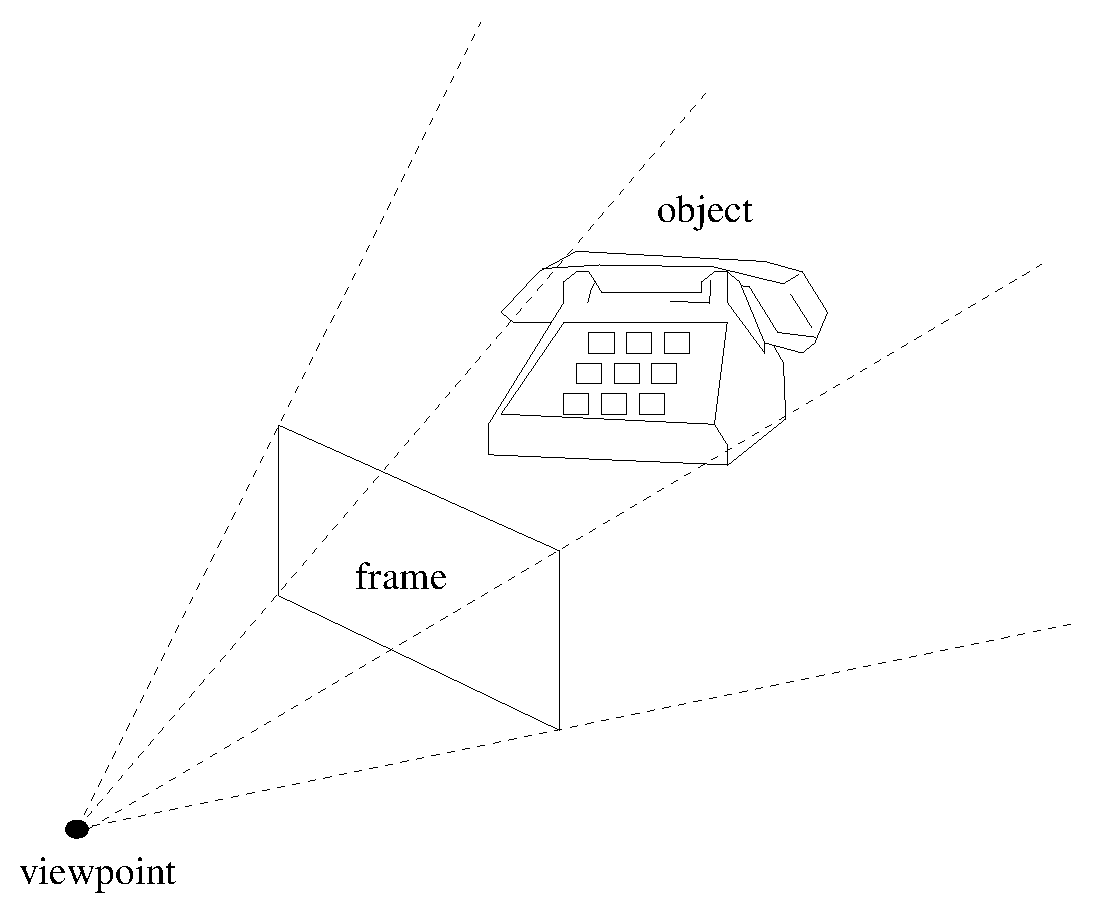
\includegraphics[width=2.3in, height=2in,angle = 0]{raytracing.ps}
\end{center}
\end{figure}
Lines ('rays') are extended from the viewpoint through a dense grid of points on the window,
and checked for intersection with the object.  If such an intersection exists, it should be 
registered as a point on the object 'visible' from the viewpoint.  In computer graphics, these 
points are projected back on the window, which becomes a 2D image that can be displayed on the
computer screen.  For our purposes, we refrain from doing this projection, and store the 
full 3D coordinates of the detected point.\\
Note that a ray may intersect the object more than once.  In these cases, the intersection point
closest to the viewpoint is chosen, as the other points are 'hidden' by it.  As mentioned above,
there are two raytracing routines in this example program.  The robust routine calculates all
possible intersection points for each ray, and then choses the nearest one.  This should always
work, but can be slow since no information is re-used.  When we have found an intersection point
for a given ray, we can usually expect that the next, neighouring ray will intersect in a point
close to the one already found.  If this is the case, it would be speedier to use a local 
algorithm that converges on the intersection point quickly given a good initial guess.  This is
the basis for our 'quick' routine.  This routine uses the robust raytracing algorithm to find
the first point on a surface, and then it switches over to the fast method as long as it is 
possible to do so.  However, since the quick method never finds more than one intersection point,
and since a ray may generally intersect an object more than once, we have no guarantee that
the point found is the one truly visible from the viewpoint.  There are some checking procedures
that make things better, but we still have no guarantee.   If the user inspects the results 
obtained, he will notice this problem even on the simple example given here.  In general, it
can be said that the rapid algorithm should only be used in some special cases, where we know
for a fact that any ray from the viewpoint will not intersect the surface more than once.\\

This is the only of the example programs that can be run with a command line argument.  If the 
first argument is \verb/q/, then the quick raytracing routine will be invoked.  Else, the
robust and slow routine is used.

\subsubsection{What it demonstrates}
\begin{enumerate}
\item The basic setting and principe of a raytracer, with a defined viewpoint, window and 
intersection with rays.
\item The use of the SISL routine \verb/s1856/, which calculates all intersections between a 
spline surface and a line.
\item The use of the SISL routine \verb/s1518/, which converges to an intersection between
a spline surface and a line, given a good initial guess.
\end{enumerate}
\subsubsection{Input/output}
The surface to be raytraced is read from the file \verb/example10_surf.g2/, generated by
the \verb/example10/ program.  The other parameters necessary for the raytracing are hard-
coded (viewpoint, view window, resolution, etc.).  The resulting points are written to the
file \verb/example15_points.g2/. 